\documentclass[12pt]{article}
%% \usepackage{bookman}
\usepackage[T1]{fontenc}
\usepackage{amsmath}
\usepackage{amsfonts}
\usepackage{amsthm}
\newtheorem*{mythm}{}
\usepackage{hyperref}
\usepackage{natbib}
\usepackage{graphicx}
\usepackage[lined, boxed, linesnumbered, commentsnumbered]{algorithm2e}
\usepackage{/home/sci/weiliu/haldefs}
\hypersetup{
  % bookmarks=true,         % show bookmarks bar?
    unicode=false,          % non-Latin characters in Acrobat’s bookmarks
    pdftoolbar=true,        % show Acrobat’s toolbar?
    pdfmenubar=true,        % show Acrobat’s menu?
    pdffitwindow=false,     % window fit to page when opened
    pdfstartview={FitH},    % fits the width of the page to the window
    pdftitle={Qual exam},
    pdfauthor={Wei Liu},     % author
    pdfsubject={Wei Liu's qual exam},   % subject of the document
    pdfcreator={Wei Liu},   % creator of the document
    pdfproducer={Producer}, % producer of the document
    pdfkeywords={qualify exam}, % list of keywords
    pdfnewwindow=true,      % links in new window
    colorlinks= true,       % false: boxed links; true: colored links
    linkcolor=red,          % color of internal links
    citecolor=blue,        % color of links to bibliography
    filecolor=magenta,      % color of file links
    urlcolor=cyan           % color of external links
}

\setlength{\oddsidemargin}{0 in}
\setlength{\evensidemargin}{0 in}
\setlength{\topmargin}{-0.5 in}
\setlength{\textwidth}{6.5 in}
\setlength{\textheight}{9 in}
\setlength{\headsep}{0.5 in}
\setlength{\parindent}{0 in}
\setlength{\parskip}{0.1 in}

\begin{document}
\title{Ph.D Qualifying Exam Answers} 
\author{Wei Liu\\ \small{(advisor: Tom Fletcher)} }
\date{\today} 
%% \maketitle 
\textbf{Ph.D Qualifying Exam Answers of Wei Liu}\hfill \textbf{March 19-26, 2012}
\hline
\hspace{6 pt}


\textbf{Question 1 (Swendsen-Wang):}

(a, b): To understand SW algorithm, some background information is needed. There
is a fundamental theorem \citep[p47]{robert2004monte} that underlies the slice
sampler and also SW algorithm. Assuming $f$ is the pdf that we want to draw
samples from, $f(x)$ can be written as
\begin{equation*}
  f(x) = \int_0^{f(x)} 1 du
\end{equation*}
$f(x)$ can be seen as the marginal distribution of joint variables $(x, u)$
\begin{equation}
(x, u) \sim \mathcal{U}\{(x,u): 0 < u < f(x)\} \label{eq:joint},
\end{equation}
where $\mathcal{U}$ is the uniform distribution, and $u$ is usually named as
\emph{auxiliary variable}. Thus, instead of  drawing samples from $f(x)$ directly
(which might be difficult), we can draw samples $(x,u)$ from their uniform joint
distribution on the constrained set $\{(x,u): 0 < u < f(x)\}$. Once we have the
samples, we can just discard $u$ and $x$ will be in original target
distribution. This is the basic idea of slice sampler.

In slice sampler, we can generate a Markov chain with the stationary
distribution equal to the joint uniform distribution of \eqref{eq:joint}. We can
generate $x$ and $u$ from their conditional distribution iteratively in a
random-walk style: 1) generate u from $\mathcal{U}(\{u:u \leq f(x))\}$, and 2)
given the new sample $u$, generate $x$ from $\mathcal{U}(\{x: f(x) \leq
u)\}$. \citet[p323]{robert2004monte} proves this Markov chain's stationary
distribution is actually \eqref{eq:joint}.

When $f(x)$ is complex function, finding the set of $x$ such that $f(x) \leq u$
can be difficult (step 2 in above procedure). Such case can happen when the $x$
is of large dimension (as in our fMRI study). The general slice sampler solves
this problem by using multiple slices. In short, $f(x)$ can be factorized into
the products of $f_i(x)$, and each $f_i$ is associated with an auxiliary
variable $u_i$. In this way, the support of the conditional distribution
$p(x|u)$ in step 2 can be easily found. The SW sampler can be seen as one of
such general slice samplers.

Here is the settings of the SW algorithm. Suppose $x$ is the set of random
variables defined on the lattice, and the probability of $x$ is defined as
\begin{equation}
p(x) \propto \exp (-U(x)), \qquad U(x) = - \sum_{(i,j)} \psi \mathbf{1}_{x_i = x_j}.\label{eq:potts}
\end{equation}
The indicator function $\mathbf{1}_{x_i = x_j}$ takes value 1 when the variables
at two spatial adjacent sites are equal $x_i = x_j$. This is a standard Potts
model. To sample from it using SW algorithm, we introduce a set of augmented
variable $u$ just like what we do in slice sampler. $u$ corresponds to the bonds
between spatially adjacent nodes. For each $u_{ij}$ between $x_i$ and $x_j$,
there are two states \emph{open} or \emph{close} denoted by $u_{ij} = 1$ or
$u_{ij} = 0$. The SW algorithm iterates between two steps
\begin{itemize}
  \item Given x, set $u_{ij} = 0$ if $x_i \neq x_j$. When $x_i = x_j$, set
    $u_{ij} = 1$ with probability $1 - \exp (-\psi)$, and set $u_{ij} = 0$ with
    probability $\exp(-\psi)$. After this step, we have multiple connected
    components, each being a subset of the nodes on the graph.
  \item Given $u$, set all the nodes in a randomly chosen cluster (i.e. a
    connect component) with same label. The label is drawn from a uniform
    distribution.
\end{itemize}
Like slice sampler, the stationary distribution of this Markov chain is the
joint distribution of $u$ and $x$, which is again a uniform distribution
\citep[ch. 6.5.2]{rubinstein2008simulation}. And it can be proved
\citep[ch. 8.2]{winkler2003image} that the marginal distribution $p(x)$ is
exactly \eqref{eq:potts}. So the joint model is consistent with the original
marginal distribution. If we sum out $x$ and get the marginal distribution of
the augmented variable $p(u)$, we have a distribution called \emph{random
  cluster model} \cite[ch. 8]{grimmett2006random}. After the sampling, we get
samples of $(x,u)$, and we just ignore the augmented variable $u$, and $x$ will
be a sample from the original Potts model.

The SW sampling is more efficient than Gibbs sampling because at each step, it
changes the labels of the whole cluster, instead of a single site. Even in low
temperature, the sampler flip the labels for larger clusters. The mixing time of
the sampling is polynomial in regular lattice.

\citep{barbu2005generalizing} talked about the convergence rate of Swendsen-Wang
(S-W) algorithm on a Potts model. They cited \citet{huber2003bounding} who
developed a new bounding chain algorithm that can diagnose the convergence of
Swendsen-Wang sampling. The number of steps to reach perfect sampling (which
means convergence to stationary distribution) is in the order of
$\mathcal{O}(\log |E|)$, where $E$ is the set of edges. This running time
applies when the temperature is far below or far above critical
temperature. \citet{cooper1999mixing} shows the mixing time (or convergence
time) is polynomial if the number of neighbors of each node does not increase
with $|V|$, the size of the nodes. This is good for regular lattice where the
number of adjacent nodes is fixed, regardless of image size. Compared with the
super-exponential rate of increase for the iteration number in standard Gibbs
sampling (see question 5 of this report), S-W algorithm is a big improvement for
convergence rate. One thing that need note is these theoretical analysis is for
the cases without external fields (data likelihood term).

(c,d): The original SW sampling only applies to Ising and Potts models, and
generalized SW sampling can be applied when there is data likelihood and we seek
sampling from posterior probability. Another disadvantage of original SW is it is
slow when sampling the labels for a cluster in step 2, since it does not use the
observed data. The last contribution of generalized SW is the adaptive increasing
or decreasing the number of labels.

There are two significant changes from standard SW to generalized SW. First, the
probability of turning on the edges (bonds) at step 1 is changed from $q_0 = 1 -
\exp (-\psi)$ to $q_e = - g(h_i, h_j)$, where $h$ is the observed data (or
features). $g(h_i, h_j)$ would takes larger value when the observed data at $i$
and $j$ are similar. The similarity is represented by the KL divergence in
\citet{barbu2005generalizing}, but can be defined differently in other
applications.  Second, The sampling of labels in step 2 could be have
acceptance rate smaller than one, instead of the 100\% acceptance in original SW
algorithm. the acceptance probability to move to new labels also depends on
posterior probability given the observed data, as shown in theorem 2 of
\citeauthor{barbu2005generalizing}.

The third version SWC-3 of the generalized SW replace the Metropolis-Hasting
sampling in step 2 with a Gibbs sampler and achieve the acceptance of 1. The
Gibbs sampler draw labels from the posterior probability given the data.

Relating to the fMRI application, there are two issue to address in order to use
SW sampling. First we need to define a function $g(h_i, h_j)$ to replace the KL
divergence in eq (12) of \citeauthor{barbu2005generalizing}. The function will
be plugged into the acceptance probability when sampling the augmented variable
$u$ (edge variables). One straightforward solution is to use the correlation
between two time courses. An edge will be open with larger probability if two
voxels connecting the edge has higher correlation. However, there is no
justification of such method. Actually, more work need to be done to find the
relationship between the acceptance probability $q_e$ and the marginal
probability $p(label | data)$.


Another issue is the sampling of labels in step 2 of the SW algorithm. Here
again we need integrate posterior probability given the data. From theorem 2, it
is possible to accept or reject a candidate label for a cluster based on the
posterior probability $p(\pi' | data)$, where $\pi'$ is a new partition of the
graph after replacing a cluster's current label with new candidate label, so it
is a \emph{candidate partition}. Put it in another way, the acceptance
probability is a function of $p(\pi' | data)$.

A comment on SW sampling: I believe the key difference is to replace prior with
posterior term in step 1. That is, instead of using $q_0$, we now use $q_e$
which is a function of observed data. From the derivation in \citep[chap
  6.5]{rubinstein2008simulation}, to use SW for sampling from posterior, it
suffice to replace prior energy with posterior energy when sampling $u$, and the
cluster label of $x$ can just be sampled from the uniform distribution, just
like the original SW algorithm. However, \citeauthor{barbu2005generalizing} uses
a different sampling method for $x$ in step 2, because that will further
increase the convergence speed. Now the sampler in step 2 will choose those
\emph{good} candidate label in the posterior sense. The SWC-3 method also serves
this purpose.

\newpage
\textbf{Question 2 (BOLD signal):} 

Information is transferred in axons between neurons by the release of
neurotransmitter molecules at synapses. The interactions between
neurotransmitter and receptors consume energy. Because energy is produced by
oxidative metabolism, increased synaptic activity will also increase local
demand for delivery of oxygen. This, counter-intuitively, increase the local
blood flow, and increases the $T_2^*$ image intensity
\citep{lewin2003functional,stroman2011essentials}. Even deoxygenated hemoglobin
decreases during neural activity, MR signal increases. This is because more
oxygen is supplied to the brain region than is consumed.

Haemoglobin have different magnetic property when it is bound to oxygen. This
changes the local distortions of a magnetic field, which can be detected by MRI
scanner. The relaxation times depends on the level of blood oxygenation, and the
MRI signal depends on the relaxation time.

To understand the response of BOLD signal to a general stimulus signal, we need
to know its response to a very short impulse signal, namely, a $\delta$
function. It is noted that the BOLD signal have about 2 seconds lags after the
onset of stimulus. This initial dip is attributed to the transient increase of
deoxygenated hemoglobin. After 4 to 6 seconds, the demand due to increase neuro
activity results in an increased inflow of oxygenated blood, and it reach the
highest point. After the neuro activity stops, the BOLD goes below the baseline
level. It takes about 20 seconds for the BOLD to go back to the baseline in this
\emph{poststimulus undershot} The balloon model \citep{buxton1998dynamics} is
used to explain this extended period. The response function to a $\delta$
function is called the \emph{Hemodynamic response function} (HRF). The response
of a general boxcar function, would be the convolution of the boxcar function
and the HRF.

\textbf{Artifactual signal in BOLD:} Since BOLD signal does not measure neural
activity directly, there might be some unwanted signal source in BOLD. First,
changes in vascular system in response to the neural activity can occur in brain
regions far from the actual activity location, initiated by flow-substances by
neurons into the extracellular space, or initiated by glial cells (which do not
directly participate neural activity)
\citep{huettel2004functional,noll2001primer}.

Another artifactual signal source is the blood vessel. Because oxygen-rich blood
flow increases dramatically to compensate the consumption of oxygen in neuronal
activity, only a small proportion of oxygen will be actually used. The
remaining hemoglobin-rich blood pass along the venous system, will increase the
BOLD signal along the downstream of the activated neurons. Such effect leads to
the question \emph{Brain or Vein}, since may reported activated regions might be
a sequence of venous drainage instead of a local neuronal activation.

A simple method to detect such signal confounds is the large magnitude change of the BOLD signal. Because of the large volume of blood vessel, BOLD signal will change in a larger magnitude due to the blood drainage. Another indicator is that the initial dip of the BOLD signal will not be observed in a blood vessel driven signal change. This is because the initial dip only happens when there is actual oxygen consumption happening in the capillaries, and will not happen at voxels containing large vessels that are distant from the active neurons. 


Electric noise is a thermal driven Brownian movement, and can happen from the
MRI coil, the electronic hardware of the scanner. Thermal noise will be
increased in a higher temperature environment. Ideally, the magnitude of thermal
noise does not depend on the voxel's spatial location. One way to increase
signal-to-noise (SNR) is to increase the $B_0$. This is because the MR signal
increase as a function of $B_0^2$, while the noise increase as a function of
$B_0$. So th SNR is roughly a linear function of $B_0$.  Another method is to
take the measurements multiple times so the noise cancels, but this does not
apply to fMRI.

System noise comes from the variations of the scanner hardware. One example is
the bias filed in MRI image. Another example is the scanner drift of fMRI. There
is a linear trend on time courses. The linear trend can be subtracted by a
detrending procedure by estimating the trend parameter.

The spatial resolution of fMRI is usually a few millimeters. If the spatial
resolution is too low, each voxel will include different tissues. This is the
\emph{partial volume effect}. If a voxel includes 50\% gray matter, 25\% white
matter, and 25\% cerebrospinal fluid, the joint effect of these tissues would
result in a intermediate value on the final voxel intensity. 

Subject head motion is another source of unrelated signals in BOLD time
course. With head motion, voxels at different time points may not correspond to
the same spatial coordinates. Also it may introduce spatial correlations since
all voxels will change at same time together. It can usually be estimated and
removed by a motion correction method, i.e. register volumes at all time points
to the first (or the middle) volume by a rigid-body transformation. Sometimes
the motion is correlated with paradigm task signal and this makes motion
correction potential dangerous since it may remove task-related signal
also. Another method to mitigate motion is to do a linear regression with head
motion parameters as explanatory variables and keep the residual signals for the
following functional connectivity analysis.

Respiration is also one of the physiological noise in the BOLD signal. One
solution is the band-pass filter that removes the signal below 0.01 Hz and above
0.1 Hz. However, if the TR is long, the breathing signal may be aliased and
difficult to remove. Cardiac signal due to the hear beat may happen throughout
the brain, but without a heart beat signal recorded together with fMRI scan, it
is hard to remove such confounds.

There are other patterns of signals in BOLD, such as intrinsic variation in the
brain due to practice, or due to fatigue, unrelated neural activity, cognitive
or behavioral variability of how the subjects performs an task, etc. The
variation between subjects can be alleviated by a group analysis with enough
number of subjects.

\newpage
\textbf{Question 3 (MMSE estimator):}

This is a Bayesian linear model, which is a Bayesian equivalent of the general
linear model. The model can be written in a matrix notation as
\begin{equation*}
\vec x = \mat H \vec \theta + \vec w,
\end{equation*}
where x is a $N\times 1$ data vector, $\mat H = [\vec h, \mathbf{1}]$ is
$N\times 2$ matrix, and $\vec \theta = [\alpha, \beta]\T$ is the parameter
vector to be estimated.

(a) The MMSE estimate of $\vec \theta$ is the posterior mean $p(\vec \theta |
\vec x)$. This can be shown by compute the derivative  of the Bayesian MSE 
\begin{equation*}
  Bmse( \vec {\hat\theta}) = \mathbb{E} [(\vec \theta - \vec{\hat\theta})^2]
\end{equation*}
with respect to $ \vec {\hat\theta}$. And the expectation is for both variable
$\vec x$ and $\vec \theta$ since both are assumed to be random in Bayesian
framework. Therefore the MMSE estimator will be
\begin{equation*}
\vec {\hat\theta} = \mathbb{E}[\vec\theta | \vec x]
\end{equation*}
Because both $p(\vec\theta)$ and $p(\vec x| \vec\theta)$ is Gaussian
distribution, the joint probability $p(\vec x, \vec \theta)$ is also Gaussian,
and also is the posterior $p(\theta|\vec x)$. Here we directly use the result
\citep[ch. 10.6]{kay1998fundamentals}
\begin{equation*}
  \mathbb{E}(\vec \theta | \vec x) = \vec \mu_\theta + \mat C_\theta \mat H\T (\mat H \mat C_\theta \mat H\T + \mat C_w)^{-1} (\vec x - \mat H \vec \mu_\theta), 
\end{equation*}
where $\mat C_\theta$ is the covariance matrix of parameter vector $\vec
\theta$. In this model, $\mat C_\theta = \sigma_\theta^2\mathbf{I}$. $\mat C_w$
is the covariance matrix of noise term $\vec w$. In our model, $\mat C_w = \mat
I$, the $N\times N$ identity matrix. Plugging into the above equation, we get
\begin{align*}
  \mathbb{E}(\vec \theta | \vec x) &= \vec \mu_\theta + \sigma_\theta^2 \mat{I} \cdot \mat H\T(\mat H \cdot \sigma_\theta^2 \mat I_{22} \cdot \mat H\T + \mat I)^{-1} (\vec x - \mat H \vec \mu_\theta),
\end{align*}
where $\mat I_{22}$ is $2\times2$ identity matrix. Using the identity $(\mat A +
\mat B \mat C \mat D)^{-1} = \mat A^{-1} - \mat A^{-1}\mat B (\mat D \mat A^{-1}
\mat B + C^{-1})^{-1} \mat D \mat A^{-1}$, we have
\begin{align*}
  (\mat H \cdot \sigma_\theta^2 \mat I_{22} \cdot \mat H\T + \mat I)^{-1} &= \mat I - \mat I \mat H(\mat H\T \mat I \mat H + \frac{1}{\sigma_\theta^2}\mat I_{22})^{-1} \mat H\T \mat I\\
  &= \mat I - \mat H(\mat H\T\mat H + \frac{1}{\sigma_\theta^2} \mat I_{22})^{-1} \mat H\T
\end{align*}
Because $\mat H\T \mat H = \begin{pmatrix}N & 0 \\ 0 & N\end{pmatrix}$, we get
\begin{align*}
  \mathbb{E}(\vec \theta | \vec x) &= \vec \mu_\theta + \sigma_\theta^2 \mat H\T(\mat I - \frac{\sigma_\theta^2}{1+N\sigma_\theta^2}\cdot \mat H \mat H\T) ( \vec x - \mat H\mu_\theta).
\end{align*}
With some simplification, we have
\begin{align}
 \mathbb{E}(\vec \theta | \vec x) &= \vec \mu_\theta + \frac{N}{N + \frac{1}{\sigma_\theta^2}}(\frac{1}{N}\mat H\T \vec x - \vec \mu_\theta), \label{eq:mmse}
\end{align}
which is the MMSE estimator of the parameter vector $\vec \theta$.

(b). If we look at \eqref{eq:mmse}, we see it is a trade-off between the prior
mean $\mu_\theta$, and the maximum likelihood (ML) estimation $\frac{1}{N}\mat
H\T \vec x$.  If the prior variance $\sigma_\theta^2$ is large (flat prior), the
Bayesian MMSE estimator will converge to the ML estimation. It is called the
likelihood \emph{swamps out} the prior. Another condition to make this happen is
when $N$ is large. Again we trust data more than the prior.

(c). The MMSE minimize the quadratic cost function, and there are other
definitions of cost function. If we define a Hit-or-miss cost function, the
posterior mode will minimize such a function. Because in our model the posterior
probability is Gaussian distribution, the posterior mean and posterior mode are
identical. Therefore, the MAP estimator is also the MMSE estimator.


\newpage
\textbf{Question  4 (Fiber tracking):}

(a). Diffusion Tensor Imaging (DTI): Water diffusion is anisotropic in white
matter. This anisotropy can be measured by Diffusion Tensor Imaging and used to
find the path of fiber tracts, and the connectivity between two region of
interests (ROIs).  The anisotropy can be represented by a diffusion
ellipsoid. In DTI, The eigenvector of the diffusion tensor with the largest
eigenvalue is assumed to align with the fiber orientation. For 3 eigenvalues
$\lambda_1, \lambda_2, \lambda_3$, if at a specific voxel $\lambda_1 \gg
\lambda_2 = \lambda_3$, the ellipsoid would be cylindrical structure along the
direction of $\lambda_1$. A straightforward approach for fiber tracking is
connecting each voxel to the adjacent voxel along the largest eigenvalue's
direction. \citet{mori1999three} propose to track a continuous rather than a
discrete vector field, and is the first DTI fiber tracking method. The
termination of fiber is judged by thresholding the fractional anisotropy value.

Flow based fiber tracking approach \citep{campbell2005flow} uses use the full
diffusion tensor as opposed the principal diffusion directions, works better
especially at in regions of partial volume. Still, the small noise of the
diffusion tensors at each voxel can accumulate after hundreds or thousands of
steps, resulting the estimated fiber deviating from the truth. Probabilistic
tracking methods \citep{basser2000vivo} are proposed to avoid this issue. At
each step, the direction is sampled from a posterior distribution, the tracking
is repeated to get multiple trajectories. A normalization step is followed to
get the spatial distribution of the fiber bundle between two ROIs.

(b). The above methods fall into the category of \emph{greedy} algorithms in
that the tracking algorithm looks for a local optimal direction at each single
step. \citet{zalesky2008dt} proposes a global optimization method that use
dynamic programming technique to find the global optimal fiber path between two
ROIs or seeds. Similar dynamic programming method are also used in
\citet{poynton2005probabilistic}, but no detailed information is available. Here
I will take \citeauthor{zalesky2008dt} as an example for the application of
dynamic programming in fiber tracking.

\citeauthor{zalesky2008dt} project the original fiber tracking problem to a new
problem of finding shortest (or minimal-cost) path on a undirected weighted
graph. A graph is defined such that each voxel is a node, and an edge is added
whenever two voxels are spatially adjacent. The weights of the edges are defined
by the diffusion tensor. That is, each edge is assigned a Bayesian posterior
probability to indicate the likelihood that the edge is aligned to the true
fiber. Between two seeds (ROIs), each possible path is assigned a probability of
the confidence that this path is the true fiber. This probability is defined as
the product of the posterior probability at each edges that it travels
through. The goal is to find a path with largest probability. This is a global
objective function and can be solved by dynamic programming method.

(c). Dynamic Programming (DP)
\citep{kleinberg2006algorithm,cormen2001introduction} is an optimization method
that combine the optimal solution of subproblem to obtain the optimal solution
of the original problem. Whenever there is a subproblem and a optimal solution
to it, we see the possible application of DP. According to
\citep{kleinberg2006algorithm}, there are a few elements in the problem that we
can apply DP:
\begin{itemize}
\item The number of subproblems should be polynomial.
\item The solution of the original problem should be easily compute from the
  solutions of the subproblem. The cost of the solution to the original problem
  is the sum of the cost of subproblems and the cost of making the choice of
  which subproblem to use for solving the original problem
  \citep{cormen2001introduction}.
\item There is natural ordering of the subproblems and recurrence that allows
  one to get the solution of a subproblem from that of a smaller subproblem.
\end{itemize}

DP is similar to divide-and-conquer method in that both split the original
problem into subproblems. However, in divide-and-conquer, the subproblems are
independent, while in DP the subproblems have overlaps, i.e., they share smaller
subproblems. In such case, divide-and-conquer will do redundant work on these
overlapping smaller subproblems. DP instead solve the common subproblems only
once and have a data structure to save these solutions. This is called
\emph{memorization}, which is a crucial component of DP. By memorization we may
achieve a polynomial-time algorithm when divide-and-conquer could not.

(d). Here we take \cite{zalesky2008dt} as example for searching the path
searching between two points $u$ and $v$ in a graph. Define the graph
$\mathcal{G} = (\mathcal{I}, \mathcal{E})$, where vertex set $\mathcal{I}$
includes all voxels in a DTI image, and edge set $\mathcal{E}$ includes any edge
$e$ if it is connected by two adjacent voxels. Assuming we already compute the
edge weights $p(e)$ for all $e\in \{\mathcal{E}_{x}\}_{x \in \mathcal{I}}$ from
the DTI images, the goal is to compute a discrete approximation $(x_0, x_1,
\dots, x_N)$ of a path with maximum probability $s^*_{u,v}$.
\begin{algorithm}[htb]
  \label{alg:alg1}
  \SetAlgoLined
  \KwData{Undirected $\mathcal{G}$, edge probabilities $p(e)$. Seed point $u$ and target point $v$. }
  \KwResult{$s*_{u,v}$}
  $d(x) := - \infty, \forall x \in \mathcal{I}$\;
  $prev(x) := empty, \forall x \in \mathcal{I}$\;
  $d(u) := 0$\;
  $\mat Q := \mathcal{I}$\;
  \While{$\mat Q$ is not empty}{
    $\mat Q := Q \textbackslash x^*$, where $d(x^*) = \mathrm{max}_{x\in\mat Q} d(x)$\; \nllabel{nl:1}
    \ForEach(){$e\in\mathcal{E}_{x^*}$}{
      \If{$d(x^*)+\log p(e) > d(x_e)$}{ \nllabel{nl:2}
        $d(x_e) := d(x^*) + \log p(e)$\;
        $prev(x_e) := x^*$\;
      }
    }
  }
  
  $x:=v, \qquad s^*_{u,v} := (v)$\; \nllabel{nl:3a}
  \While{$x\neq u$}{ 
    $x:=prev(x)$ \nllabel{nl:3}
    Add x to the head of $s_{u,v}^*$\;
  }
  \caption{Dijkstra's algorithm for shortest path (maximum probability) search. }
\end{algorithm}

Algorithm \ref{alg:alg1} gives the Dijkstra's algorithm for shortest path
search. Here we have minor modification to apply it for maximum probability
search for path between source $u$ and target $v$. In this algorithm $d(x)$ is
the maximum probability between $u$ and $x$. $d(x)$ is initialized to
$-\infty$. $prev(x)$ is the previous node of $x$ along the path from $u$ to $v$,
and is initialized to empty. The algorithm also maintain a subset of vertex
$\mat Q$ for those that have not been explored (i.e. have not been computed for
$d(x)$). At the beginning, $\mat Q$ includes all nodes in the graph. After the
node has been explored, it is removed from $\mat Q$ (line \ref{nl:1}). $\mat Q$
uses a special data structure (priority queue) that can extract minimal value of
$d(x)$ fast. When a $x$ with minimal value of $d(x)$ is extracted, its
adjacent neighbors $x_e$ are explored by updating $d(x_e)$ (line
\ref{nl:2}). This is done until $\mat Q$ is empty, that is, all nodes are
explored.

A shortest path from $u$ to $v$ can be easily found by back searching the
previous node of x at line \ref{nl:3} until the head node reaches source node
$u$.


There are few things that is worth noting. First, standard Dijkstra's algorithm only
applies to graph with positive weight on all the edges, while the Bellman-Ford
algorithm can be used to general with negative edge weights, but with a slower
running time \citep[ch 24]{cormen2001introduction}.  In our graph of DTI image,
the edge weights  $\log p(e)$ is negative. However, this is not a problem
for Dijkstra's algorithm since here we look for maximum probability of a
path with all negative edge weights, which is equivalent to finding the minimal cost or shortest path with all positive edge weights.

Another thing is the implementation in \ref{alg:alg1} is not yet a dynamic
programming approach (algorithm the author claims so), since it does not use DP
concept, i.e. the memorization of the overlapping part of subproblems. This is
not a problem as DP does not necessarily outperform greedy algorithm for all
problems. Algorithm $\ref{alg:alg1}$ is similar to the Breath-First-Search which
is a greed algorithm. Not all greedy algorithm can achieve the optimal solution
but Dijkstra's algorithm can achieve it with a polynomial time, and is even
faster than the dynamic programming version of the path-searching algorithm
below.

The dynamic variants of shortest path search is due to Bellman-Ford
algorithm. To give a sketch of the algorithm, think again splitting the optimal
solution into subproblems. Assume \textsf{OPT(i,v)} si the minimum cost of a
path from $i$ to $v$, the recursive formula used for DP can be written as
\citep[chap 6.8]{kleinberg2006algorithm}
\begin{mythm}
  if $i > 0$ then $OPT(i,v) = min(OPT(i-1, v), min_{w\in V}(OPT(i-1,w) + c_{vw}))$,
\end{mythm}
where $V$ is vertex set, and $c_{vw}$ is the cost of edge $(v,w)$. If we assume
the number of vertex (voxels) in the graph is $n$, and the number of edges is
$m$, constructing a dynamic programming table in $\mathcal{O}(n^3)$ time, so the DP
shortest path finding algorithm takes $\mathcal{O}(n^3)$ time to finish. A basic
improvement of the algorithm is possible when the edges are close to $n^2$ (our
DTI image even has much less edges), and have a running time
$\mathcal{O}(nm)$. This seems still worse than the best Dijkstra algorithm with
careful implementation of the priority queue on the $\mat Q$.

To see the difference of the path search between a 2D image and 3D volume, we
see there is really no difference except of the increasing number of data
points. To choose from different variants of the Dijkstra's algorithm, one may
need to know the number of edges compared to the number of vertex. For 2D
regular lattice image, each pixel can be seen to have 4 neighbors. We will have $m = 2n$ in such case. For 3D volume with standard
6-neighborship, $m = 3n$. Either way $m$ is the linear function of $n$, so the
graph can be seen as sparse.

(e). How fast is the Dijkstra's algorithm? The algorithm loops all $n$
nodes. For each notes, it will reach all of its adjacent nodes to compute the
minimal(maximal) value at line \ref{nl:2} of algorithm \ref{alg:alg1}. For a
graph with $m$ edges, computing these minima will take $\mathcal{O}(m)$ time, so
it will take $\mathcal{O}(nm)$ time at most to finish the Dijkstra's algorithm.

For regular lattice in DTI volume, $m\approx 3n$, so it is a sufficiently sparse
graph, and the upper bound of the running time is tighter than
$\mathcal{O}(nm)$.  The running time of Dijkstra's algorithm depends on the
implementation of the min-priority queue of $\mat Q$, and can be as low as
$\mathcal{O}(m)$ time plus the time for $n$ \textsf{extractMin} and $m$
\textsf{ChangeKey} operations \citep[chap 4.4]{kleinberg2006algorithm}.  If we
implement the queue as a binary min-heap, the running time will be
$\mathcal{O}(m\log n)$ \citep[chap 24.3] {cormen2001introduction}.

(f). Parallel implementation of Dijkstra's algorithm has been available since
\citet{nepomniaschaya2000simple}, but it is \citet{harish2007accelerating} that
gives a implementation of the algorithm on Nvidia GPU platform. Two GPU kernel
function is implemented to update the current short path data structure
(i.e. the $d(x)$ in algorithm \ref{alg:alg1}) to avoid the read after write
inconsistencies, the speedup is shown in figure \ref{fig:gpu}. It can be seen
that the GPU version of the path-searching implementation has significant speedup
compared to the CPU version, which means the fiber tracking on GPU is a
promising research direction. Even more speed up can be shown in a newer
implementation of \citet{buluē2010solving}, who has extensively use of matrix
multiplication and thus has a high ratio of computation to communication.
\begin{figure}
  \centering
  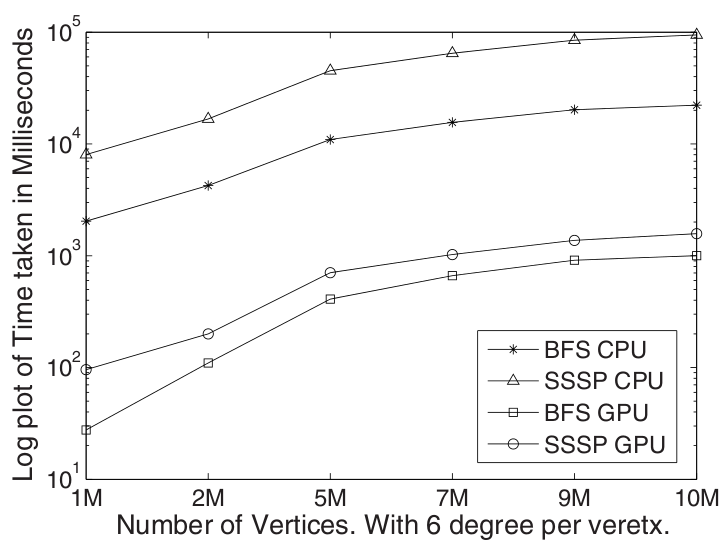
\includegraphics[width=0.5\textwidth]{gpu}
  \caption{Compare the speedup of path search on GPU (SSSP) with CPU. BFS is the
    standard breath-first-search algorithm. Figure is from \citet{harish2007accelerating}. }
  \label{fig:gpu}
\end{figure}

(g). Before answer the question, we need a classification of fiber tracking
algorithms. These algorithms are usually \emph{single-path fiber tracking
  algorithms} and \emph{all-paths fiber tracking problems}. The former find
shortest (or most probable) path between know seed point $u$ and end point
$v$. The latter finds shortest paths starting from seed point $u$ and ending to
unknown target point. All-path approaches are often used to find a \emph{probabilistic} path beginning from a seed point. 

The Dijkstra's algorithm can be used to find the all-paths as well as single
path by same routine. This is because as a breath-first-search algorithm,
finding the all-paths need the same amount of computation with finding the
single-path. 

Now for all-path searching , the seed and target point are both on surface of
the 3D volume. I believe this does not have effect on the computation time of
Dijkstra's algorithm. this is because as a breath-first-search algorithm,
Dijkstra's algorithm may still have to explore all data points in the volume,
even at last we only choose those shortest paths with ending point on the
surface. If we apply algorithm \ref{alg:alg1} to all-path searching, the
constraints that the ending points is on the surface only have effect on the set
of $v$ from which we want to back reconstruct the path.  Because the
back-searching of line \ref{nl:3a} is linear time, changing of this piece does
not change the upper bound of the Dijkstra's algorithm.

If, on the other hand, we want to find the all-pair shortest path between each
pair of voxels in the volume, the constraint of starting and ending points on
surface have larger impact on the running time. Without the constraint, We can
run Dijkstra's algorithm for each $u\in\mathcal{I}$. Because Dijkstra's
algorithm with binary min-heap implementation is $\mathcal{O}(m\log n)$, the
running time for all-path shortest path searching will be $\mathcal{O}(mn\log
n)$. With the constraints that $u\in \mathcal{I}_s$, where $\mathcal{I}_s$ is
the set of the points on the surface, the running time of all-pair searching
will be $\mathcal{O}(|\mathcal{I}_s| m\log n)$, where $|\mathcal{I}_s|$ is the
number of points on the surface.

A side note: I am thinking whether the global energy function is really optimal
in the application sense. Suppose that we are looking for the global-optimal
path from $u$ to $v$. If the fiber tract we find pass through point $x$ and $y$,
and the probability of the sub-path between $x$ and $y$ is very low. We may
argue even this path $(u,v)$ maximize the global probability, the \emph{broken}
segment between $x$ and $y$ make me think the path $(u,v)$ is not the optimal
path in the real application. So, we may need a constraint: we do not want a
path such that any segment of which has probability below certain threshold. If
that happens, the fiber tract is believed to be broken and will not be the
optimal solution. Finding the shortest path with constraints has been discussed
in the literatures, and can be used for such problems.

\newpage
\textbf{Question 5 (Gibbs Sampling Convergence):}

(a) If the staring point of the Markov chain is poorly chosen, the burn-in
period will increase dramatically. The rule of thumb is choosing the staring
sample close to the center of the distribution, i.e., the mode of the pdf. The
proposal distribution of the Metropolis-Hasting sampling also has big impact on
the steps needed to reach stationary distribution. For example, the random
walker, a special case of Metropolis-Hasting sampler, has a symmetric proposal
distribution (either uniform, or Normal distribution) with a tunable variance
parameter. Increasing this variance parameter will have larger movement which is
good to explore the whole support space, but at the risk of low acceptance rate
and high correlation between samples. If the variance is too small, there are
higher probability of accepting the candidates, but less opportunity to explore
all modes of the target distribution, and the samples are also highly
correlated. In such case, the chain will converge too slowly.

 (b,c). Perhaps the single most popular approach is due to
\citet{gelman1992inference}. To use their method, we need to run multiple
parallel MCMC chains with different starting points. These chains must be
overdispersed initially with respect to the posterior. Each chain has length
$2N$ and the first half of points are discarded. If we use $\psi_{mn}$ to
represent the statistics of chain $m$ at time $n$.  The Gelman-Rubin method
compute the between and within-sequence variances of the statistics $\psi$
\begin{align*}
  B &= \frac{N}{M-1}\sum_{m=1}^{M}(\overline\psi_{m} - \overline \psi)^2\\
  \overline\psi_m &= \frac{1}{N}\sum_{n=1}^N\psi_{mn}, \qquad \overline\psi = \frac{1}{M}\sum_{m=1}^M\overline\psi_m\\
  s_m^2 &= \frac{1}{N-1}\sum_{n=1}^N(\psi_{mn} - \overline\psi_m)^2\\
  W &= \frac{1}{M}\sum_{m=1}^M s_m^2
\end{align*}
We can estimate the marginal posterior variance of the statistics $\psi$ by a weighted average of $W$ and $B$
\begin{equation}
 \widehat {Var}(\psi|data) = \frac{N-1}{N}W + \frac{1}{N}B \label{eq:var}
\end{equation}
This estimator overestimates the marginal variance when the staring points of
the chain are overdispersed, but is unbiased when $n\rightarrow \inf$. On the
other hand, the within-variance $W$ will under-estimate the variance of $\psi$
and converge to $Var(\psi)$ when $n\rightarrow\inf$. So we can compare the value
of \eqref{eq:var} with $W$. If they are very different, that means the chain is
not converged yet. The Gelman-Rubin uses the estimated potential scale reduction
\begin{equation*}
  \widehat R = \sqrt{\frac{\widehat{Var}(\psi|data)}{W}},
\end{equation*}
which declines to 1 as $n\rightarrow\inf$.  

One issue with this method is to get overdispersed starting points, one need have
some knowledge of the pdf of interest, for example, the modes and shape of high
density regions. If multiple chains all start from a single mode of the density
function, they may take long steps (if ever possible) to explore other modes. In
such case, multiple chains do no help much compared to a single long chain, and
the Gelman-Rubin method can not verify the convergence to the stationary
distribution.


The Gelman-Rubin method is difficult to apply to sampler high dimensional random
vectors, because saving multiple independent chains will require large memory,
and sampling these chains also have high computation cost.

The second test for convergence is a non-parametric test. It is applied to the
single chain. Assume $\theta^{(t)}$ is the statistics derived from the chain of
$1, \dots, t$. When the chain reaches stationary, $\theta^{(t_1)}$ and
$\theta^{(t_2)}$ has same marginal distribution for any $t_1$ and $t_2$. Given a
MCMC chain $\theta^{(1)}, \cdots, \theta^{(T)}$, we can compare the empirical
distributions of two half chain $(\theta_1^{(1)}, \dots, \theta_1^{(T/2)})$ and
$(\theta_2^{(T/2)}, \dots, \theta_2^{(T)})$. The Kolmogorov-Smirnov statistics
is defined as the supremum of the absolute value on the difference of two
empirical distribution functions
\begin{equation*}
  K   = \sup_{\eta} | F_1(\eta) - F_2(\eta) | = \frac{1}{M}\sup_{\eta} \left | \sum_{m=1}^M \Ind_1(\eta) - \sum_{m=1}^M \Ind_2(\eta)\right |,
\end{equation*}
where $F_1$ and $F_2$ is $\theta$'s empirical distribution for two half chains,
and $\Ind$ is indicator function. It is noted that because of the correlation
between adjacent samples in MCMC, the half chain $\theta$ is sampled in a batch
mode, i.e. $\theta_1^m$ and $\theta_1^{m+1}$ are separated by a interval to make
a quasi-independent chain. 

Under the stationary assumption, the limiting distribution of $\sqrt{M}K$ has
the cdf \citep[chap 12.2] {robert2004monte}
\begin{equation*}
  R(x) = 1 - \sum_{k=1}^{\infty} (-1)^{k-1} \exp \{ -2 k^2 x^2\}.
\end{equation*}
Now we can construct a hypothesis, with the null hypothesis as the two chains
are from same distribution (i.e., the MCMC chain reaches stationary). The hull
hypothesis is rejected if $\sqrt{M}K > K_{\alpha}$, where $K_{\alpha}$ is
computed from $\Pr(x < K_{\alpha}) = 1 - \alpha$.

It is not straightforward to generalize the Kolmogorov-Smirnov test into higher
dimension, especially for Ising model with dimension as the number of image
voxels. From Wikipedia, this is because the maximum difference between two joint
cumulative distribution functions is not generally the same as the maximum
difference of any of the complementary distribution functions. One solution is
to compare the cdfs of the two samples with all possible orderings, and take the
largest of the set of resulting K-S statistics. In $d$ dimensions, there are
$2^{d-1}$ such orderings, which is intractable for Ising model.


(d). To test the convergence of a Gibbs sampler on a simple MRF such as a Ising
model, we can instead compute the upper bound of the number of samplings. One
method is to use the coupled sampled paths to study the convergence property
\citep{johnson1996studying}. Two coupled process have same transition kernel but
different starting point. The coupled paths reach the same state after certain number
of iterations. The iteration is defined as the sweep of all the data points in
the mode.  By examining the distribution of the iterations need for coupling,
convergence properties of the sampling can be
established. \citeauthor{johnson1996studying} use a $64\times64$ regular lattice
and assume a Ising model on the binary variables on the lattice. He tried to
look for the relationship between the number of required sampling iterations and
the Ising parameter $\beta$. Figure \ref{fig:ising} shows when $\beta$ is small
the required number of iterations is also small. However, because the growth of
the iteration number is super-exponential, large value of $\beta$ will need much
more iterations to converge. When $\beta=0.9$, the 95th and 99th quantile of the
iterations distribution reached 1 million.

\citet{gibbs2000bounding} also gives a upper bound of the iterations of Gibbs
sampling on a one dimension Ising model. His upper bounds, however, is also a
function of the square of data points, and of a tolerance $\varepsilon$, on the
variation distance. Similar to \citeauthor{johnson1996studying}, the upper bound
increase fast with $\beta$. For $\varepsilon = 0.01$, $\beta=0.5$ gives a upper
bound $128N^2$, while $\beta=1.5$ gives $6162N^2$, where $N$ is number of points
in the lattice. \citeauthor{gibbs2000bounding} noted that there is no phase
transition in this 1-D model. For higher dimensional Ising model, his upper
bounds only applies to small $\beta$, and Convergence is slow when $\beta >
\beta_0$, where $\beta_0$ is the reciprocal of the critical temperature. For a
higher dimension of Ising model such that the number of neighbors of each data
points increases, the convergence upper bound even increase faster. Actually the
upper bound is a function of $n$, the number of neighbors of each node, and will
increase when $n$ increases.

As a side note, \citep{barbu2005generalizing} talked about the convergence rate
of Swendsen-Wang (S-W) algorithm on a Potts model. This is related to question 1
in this Qualify exam. They cited \citet{huber2003bounding} who developed a new
bounding chain algorithm that can diagnose the convergence of Swendsen-Wang
sampling. The number of steps to reach perfect sampling (which means convergence
to stationary distribution) is in the order of $\mathcal{O}(\log |E|)$, where
$E$ is the set of edges. This running time applies when the temperature is far
below or far above critical temperature. \citet{cooper1999mixing} shows the
mixing time (or convergence time) is polynomial if the number of neighbors of
each node does not increase with $|V|$, the size of the nodes. This is good for
regular lattice where the number of adjacent nodes is fixed, regardless of image
size. Compared with the super-exponential rate of increase for the iteration
number in standard Gibbs sampling, S-W algorithm is a big improvement for
convergence rate. One thing that need note is these theoretical analysis is for
the cases without external fields (data likelihood term). 

\begin{figure}
  \centering
  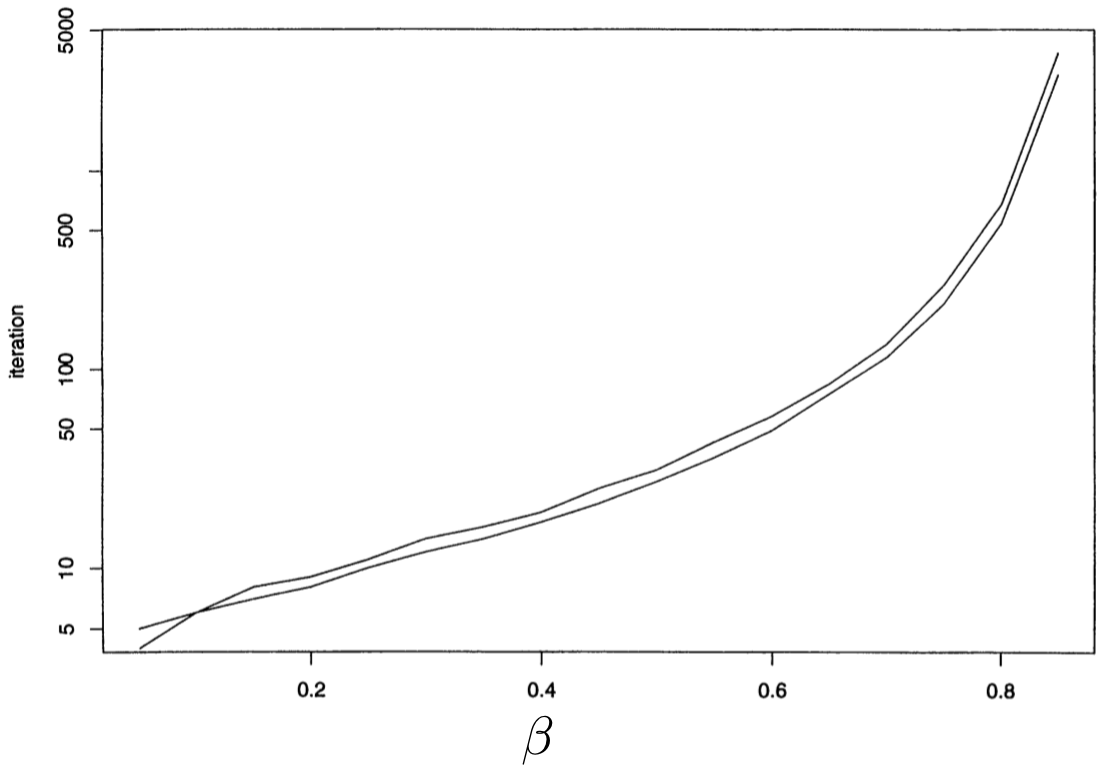
\includegraphics[width=0.7\textwidth]{ising}
  \caption{Percentile of coupling iterations for Ising model of size $64\times
    64$. Top curve shows the 99\% and bottom shows the 95\% percentile from the
    distribution of the iterations needed for coupling, as a function of $\beta$
    parameter.  The percentiles are estimated using 1000 repetitions of Gibbs
    sampling initialized with all white and all-black value. Figure from
    \citet{johnson1996studying}. }
\label{fig:ising}
\end{figure}

\bibliographystyle{plainnat} 
\bibliography{quaref}
\end{document}
